\documentclass[dcc,uchile,sol]{fcfmcourse}
\usepackage{teoria}
\usepackage[utf8x]{inputenc}
\usepackage{amsmath}
\usepackage{amsfonts,setspace}
\usepackage{listings}
\usepackage{hyperref}
\usepackage{color}
\usepackage{tikz}



\definecolor{pblue}{rgb}{0.13,0.13,1}
\definecolor{pgreen}{rgb}{0,0.5,0}
\definecolor{porange}{rgb}{0.9,0.5,0}
\definecolor{pgrey}{rgb}{0.46,0.45,0.48}

\lstset{language=Java,
  showspaces=false,
  showtabs=false,
  breaklines=true,
  showstringspaces=false,
  breakatwhitespace=true,
  commentstyle=\color{porange},
  keywordstyle=\color{pblue},
  stringstyle=\color{pgreen},
  basicstyle=\ttfamily,
  moredelim=[il][\textcolor{pgrey}]{$ $},
  moredelim=[is][\textcolor{pgrey}]{\%\%}{\%\%}
}

\newenvironment{codebox} {\small \ttfamily \obeylines \begingroup \setstretch{-2.4}} {\endgroup}

\newcommand{\ptitle}[1]{\underline{\textbf{#1}}}

\title{Auxiliar 5 - Listas y Árboles}
\course[CC3001]{Algoritmos y Estructuras de Datos}
\professor{Nelson Baloian}
\professor{Patricio Poblete}
\assistant{Gabriel Azócar, Manuel Cáceres}
\assistant{Michel Llorens, Sergio Peñafiel}


\begin{document}
\maketitle

\vspace{-1ex}


\begin{problems}
\problem \ptitle{Lista enlazada}
\newline

\begin{figure}[h]
    \centering
    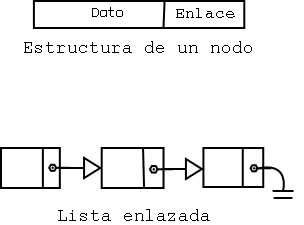
\includegraphics[width=8cm]{imagenes/lista.png}
\end{figure}

\begin{enumerate}
    \item Defina una clase ListaEnlazada que represente una lista enlazada de Strings. Su constructor debe recibir un String y tomarlo como valor, dejando el enlace como null.
        
    \item Escriba un método que reciba otra ListaEnlazada, y las una.
    
    \item Escriba un método que retorne la cantidad de valores que contiene la lista.
    
    \item Escriba un método que permita obtener el elemento i-esimo de la lista. Si sobre pasa el largo de la lista, entrega null.
    
    \item Escriba un método que permita saber si un String está contenido en la lista. Debe retornar la posición del elemento en la lista y -1 si no está.
    

\end{enumerate}

\problem \ptitle{Inventario}

Una empresa produce cada mes 20 unidades de un producto, el producto enfrenta demanda que cambia mes a mes y esta dada por $D(t) = \lfloor 5 - t + t^2/16 \rfloor$. Si un mes la empresa produce más de lo que vende entonces envía sus productos a un inventario. Al comienzo del proceso el inventario está vacío.

\begin{enumerate}
    \item Plantee una ecuación de recurrencia para el inventario. Discuta la factibilidad de obtener una solución analítica.
    \item Cree la función \texttt{int inventario(int t)} que retorna la cantidad de productos que hay en el inventario en el mes t. Para esto debe utilizar una lista enlazada global donde almacenará la cantidad de productos del inventario, en caso que se pida un valor que está en la lista debe retornarlo inmediatamente, si no está debe actualizar la lista agregando los nodos faltantes hasta obtener el valor pedido.
\end{enumerate}

\problem \ptitle{Reflejo}\\
Suponga que tiene la siguiente clase que representan los nodos de un árbol:
\begin{lstlisting}
private class Nodo{
        int valor;
        Nodo izquierda;
        Nodo derecha;

        public Nodo(int valor){
            this.valor = valor;
        }
}
\end{lstlisting}
\begin{enumerate}[a)]
    \item Cree la clase \texttt{Arbol} con su constructor y un método \texttt{agregar}, que agregue un número al árbol respetando la condición de árboles de búsqueda.
    \item Cree el método \texttt{reflejar} que cambie el árbol convirtiéndolo en su reflejo, es decir, para todos los nodos del árbol, su hijo izquierdo pasa a ser el derecho y viceversa.
    \item Cree el método \texttt{sonIguales(Arbol arbol)} que retorna \texttt{true} si ambos árboles son iguales, es decir, tienen la misma estructura y los mismos valores en los nodos.
\end{enumerate}

\end{problems}
\end{document}
